%%%%%%%%%%%%%%%%%%%%%%%%%%%%%%%%%%%%%%%%%%%%%%%%%%%%%%%%%%%%%%%%%%%%%%%%%%%%%%%%
% Copyright 2019 Louis Paternault --- http://snt.ababsurdo.fr
%
% Publié sous licence Creative Commons Attribution-ShareAlike 4.0 International (CC BY-SA 4.0)
% http://creativecommons.org/licenses/by-sa/4.0/deed.fr
%%%%%%%%%%%%%%%%%%%%%%%%%%%%%%%%%%%%%%%%%%%%%%%%%%%%%%%%%%%%%%%%%%%%%%%%%%%%%%%%

% Pour compiler :
%$ lualatex $basename

\documentclass[tikz]{standalone}

\begin{document}

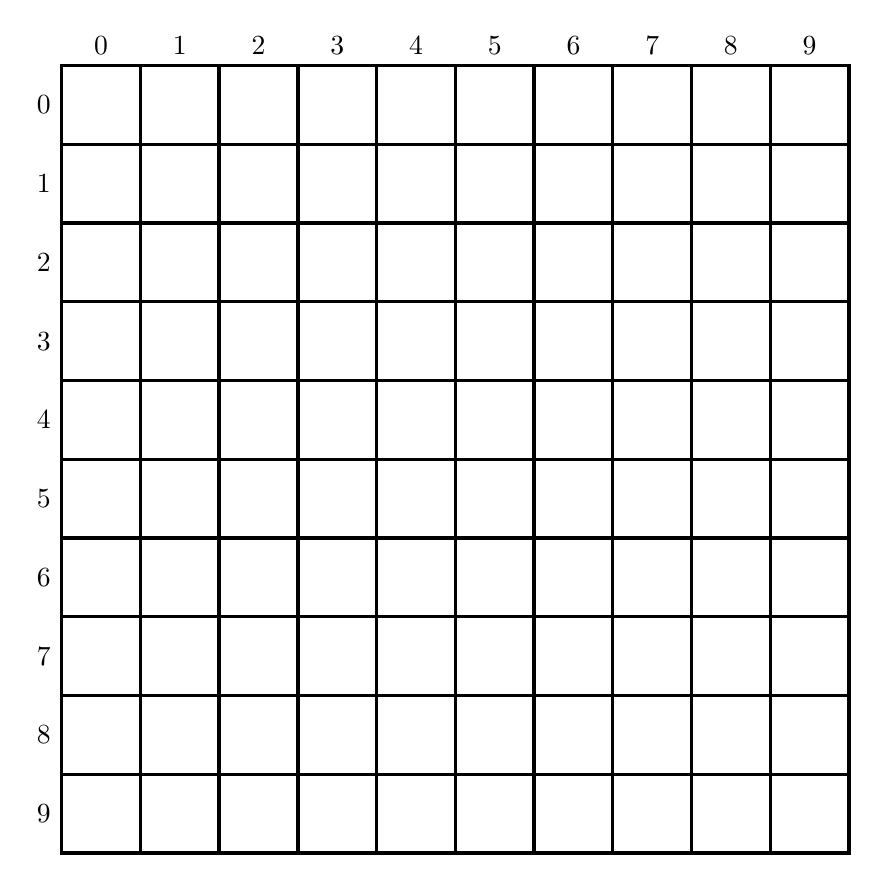
\begin{tikzpicture}[very thick]
  \fill[white] (0, 0) rectangle (10, 10);
  \draw (0, 0) rectangle (10, 10);
  \foreach \x in {0, ..., 9} {
    \draw (\x, 0) -- ++(0, 10);
    \draw ({\x+.5}, 10) node[above]{$\x$};
  }
  \foreach \y in {0, ..., 9} {
    \draw (0, \y) -- ++(10, 0);
    \draw (0, {9.5-\y}) node[left]{$\y$};
  }
\end{tikzpicture}

\end{document}
